\subsection{Charge density plots}

	\subsubsection{Helium Atom}
		For the Helium atom we have ran simulations, with \(10^6\) Monte Carlo cycles, of several different trialfunctions and recorded the position of the electrons. We first did an experiment with the electrons being in a pure hydrogenlike wavefunction, then we ran an hydrogenlike wavefunction but optimized the \(\alpha \) value to get a better ground state energy then at last we also included a Pàde-Jastrow correlation factor to include the effects of the electron-electron repulsion. For the pure hydrogenic wavefunction we got $E = -2.757$ and $\sigma^2_* = 0.0030$, while with the optimized \(\alpha\) value we got $\alpha = 1.65$, $E = -2.843$ and $\sigma^2_* = 0.0027$, and lastly with the Pàde-Jastrow factor we got $\alpha = 1.843$, $\beta = 0.34$, $E = -2.887$, $\sigma^2_* = 0.0010$. Here $\sigma^2_*$ is the variance for the local energy between each particle move in the VMC, not the true variance, which is obtained through the blocking routine described in \cref{sec:blocking}. In figure \ref{fig:HeliumChargeDensity} we plots of the positions the electrons occupied during the simulations and we can see that for the pure hydrogenic wavefunction the electrons was generally closer to the nucleus than in the other two simulations. The ground-state energy improved and got closer to the reference value \ref{tab:energyReference1} as the wavefunction got more sophisticated as well as the variance decreasing. In the wavefunction the $\alpha$ parameter represents the electrical attraction of the nucleus on the electron, and is equal to the charge in a Hydrogen atom, in a real Helium atom the attraction felt is smaller than the charge of the nucleus since there is also the effect of the other electrons. This is why we get a better simulation with a smaller \(\alpha\) value. For the Helium atom the effect of the correlation factor is not very pronounced, since the electrons can quite far away from each other, but it is still significant in the ground-state energy and the variance.
		\begin{figure}
				\centering 
				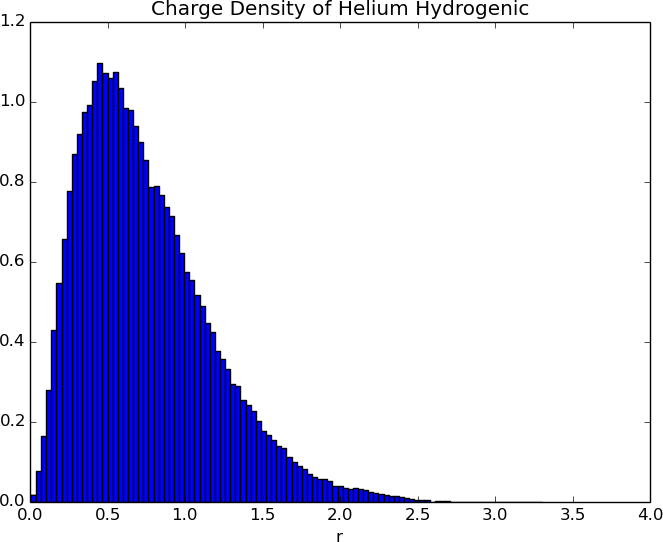
\includegraphics[width=0.32\linewidth]{../figures/used/ChargeDensityHeliumHydrogenic}
				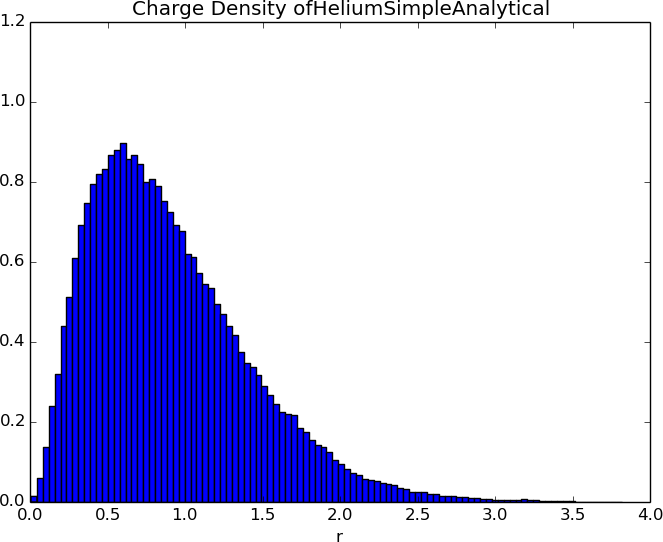
\includegraphics[width=0.32\linewidth]{../figures/used/ChargeDensityHeliumSimpleAnalytical}
				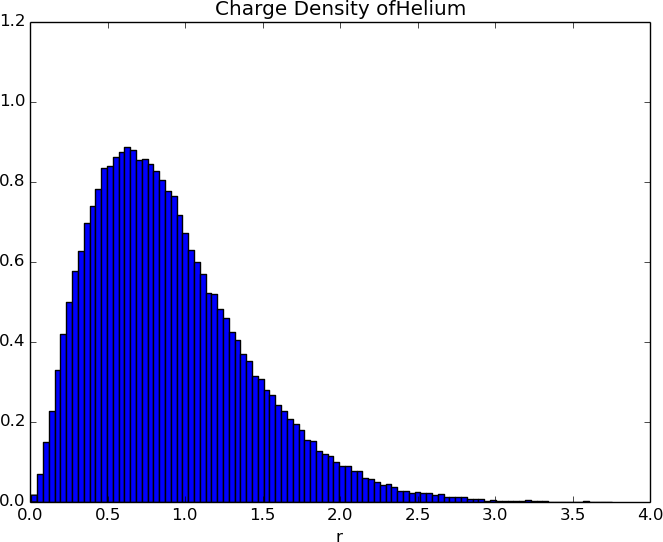
\includegraphics[width=0.32\linewidth]{../figures/used/ChargeDensityHelium_trimmed}
				\protect\caption{The electron-nucleus distance in an Helium atom simulated with different trialfunctions. From the left the plots represents pure hydrogenic wavefunctions ($\alpha = 2$, $E = -2.757$ and $\sigma^2_* = 0.0030$), hydrogenic wavefunctions with an optimized alpha ($\alpha = 1.65$, $E = -2.843$ and $\sigma^2_* = 0.0027$) and hydrogenic wavefunctions with a Jastrow factor and optimized parameters, ($\alpha = 1.843$, $\beta = 0.34$, $E = -2.887$, $\sigma^2_* = 0.0010$ ). The simulations were run with \(10^6\) Monte Carlo cycles.}
				\label{fig:HeliumChargeDensity}
		\end{figure}

		As expected since the trialfunctions used here is based only on the \(\psi_{1S}\) orbitals the radial distribution is similar to the \(\psi_{1S}\) hydrogen orbital in \cref{fig:orbitals_radial}.


	\subsubsection{Beryllium}
		With the hydrogenic Beryllium trialfunction we got an ground-state energy of \(-13.710\) with a $\sigma^2_* $ of $ 0.0072$, when the correlation factor was included the energy dropped to $-14.385$ with a $\sigma^2_* $ of $0.0029$.
		The hydrogenic wavefunction consists for Beryllium is made up of a Slater determinant constructed of the first two hydrogenic orbitals, plotted in \cref{fig:orbitals_radial}. The traces of the \(1S\) orbital is there in the first maximum and is closer to the nucleus than in an hydrogen atom, which is expected since the distance is a function of the nucleus charge, the contribution from the second orbital \(2S\) is visible as the second maximum in the distribution \cref{fig:chargeDensityBeryllium}. When the correlation factor is included the distribution is smeared out and the orbitals are not as sharp.


		\begin{figure}
			\centering 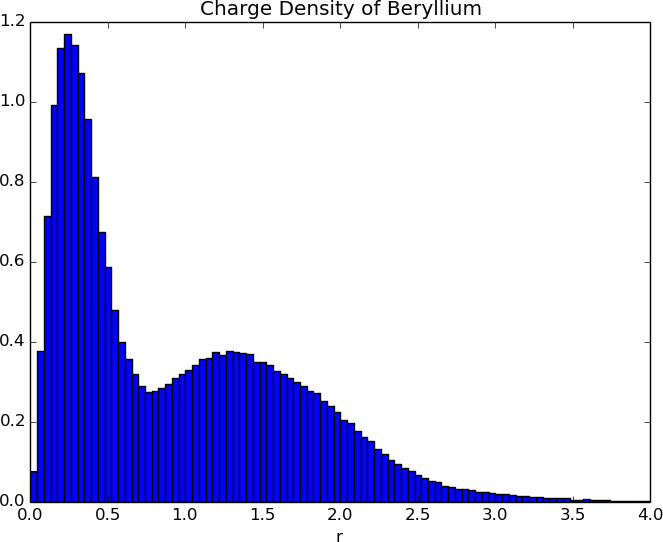
\includegraphics[width=0.45\linewidth]{../figures/used/ChargeDensityBerylliumSimple}
			\centering 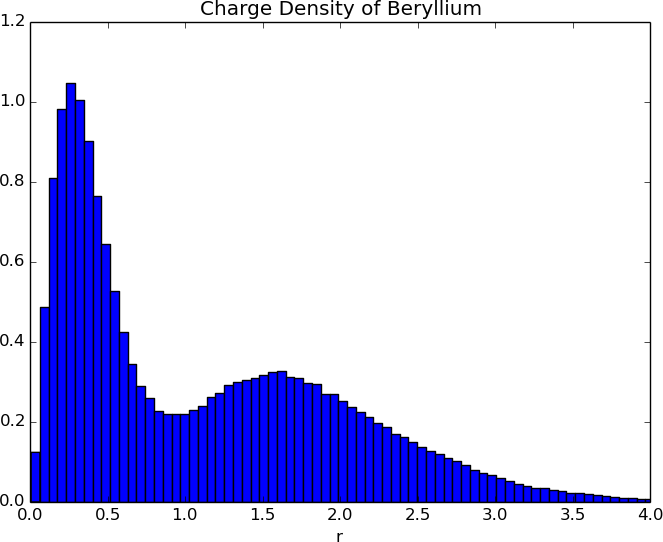
\includegraphics[width=0.45\linewidth]{../figures/used/ChargeDensityBeryllium}
			\protect\caption{The electron-nucleus distance in an Beryllium atom simulated with different trialfunctions. The left plot is with hydrogenic wavefunctions ($\alpha = 4$, $E = -13.710$, $\sigma^2_* = 0.0072$) and the right plot is withhydrogenic wavefunctions with a Jastrow factor and optimized parameters, ($\alpha = 4$, $\beta = 0.31$,  $E = -14.385$, $\sigma^2_* = 0.0029$ ). The simulations were run with \(10^6\) Monte Carlo cycles.}
			\label{fig:chargeDensityBeryllium}
		\end{figure}

		
	\subsubsection{Neon}
		The ground state energy and the \(\sigma_*^2\) got much better with the correlation factor included, from \(-110.301\) to \(127.888\) for the energy and  \( 0.0477 \) to \( 0.0190 \) for the estimation of the variance. The trialfunctions include all the three orbitals and the distribution is contracted closer to the nucleus than in the other atoms. Here we can see the largest effect due to the inclusion of the correlation factor, both in the ground-state energy and the radial distribution. This is because the electrons are closer together than in the other atoms due to the higher charge of the nucleus.
		\begin{figure}
			\centering 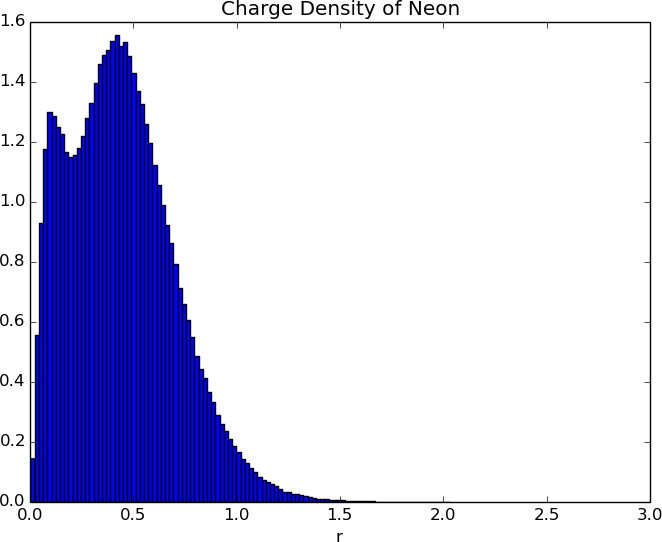
\includegraphics[width=0.45\linewidth]{../figures/used/ChargeDensityNeonSimple}
			\centering 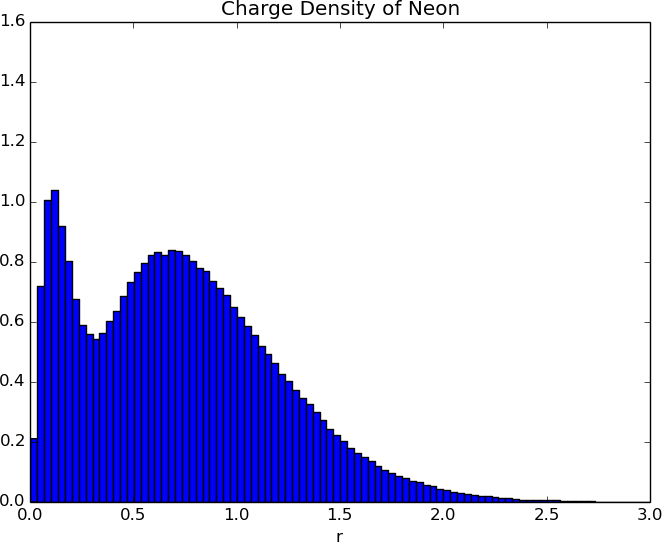
\includegraphics[width=0.45\linewidth]{../figures/used/ChargeDensityNeon}
			\protect\caption{The electron-nucleus distance in an Neon atom simulated with different trialfunctions. The left plot is with hydrogenic wavefunctions ($\alpha = 10.22$, $E = -110.301$, $\sigma^2_* = 0.0477$) and the right plot is withhydrogenic wavefunctions with a Jastrow factor and optimized parameters, ( $\alpha = 10.22$, $\beta = 0.0.091$,  $E = -127.888$, $\sigma^2_* = 0.0190$ ). The simulations were run with \(10^6\) Monte Carlo cycles.}
			\label{fig:chargeDensityNeon}
		\end{figure}

	\subsubsection{Hydrogen Molecule}
		\textbf{To be written tomorrow}
		\begin{figure}
			\centering 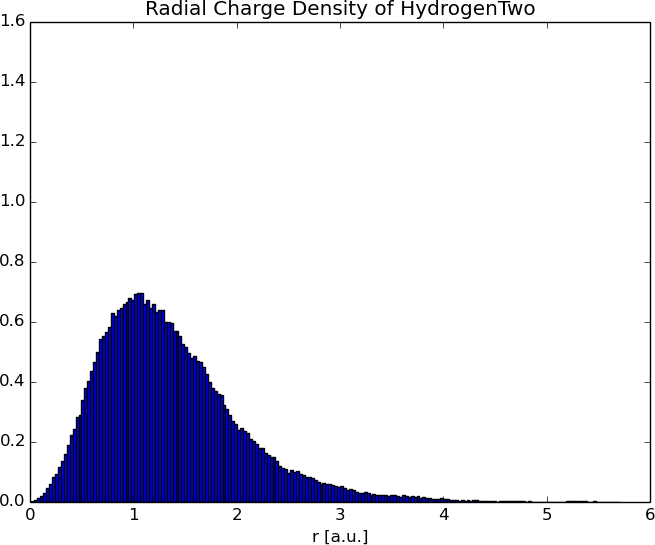
\includegraphics[width=0.45\linewidth]{../figures/used/ChargeDensityHydrogenTwo}
			\centering 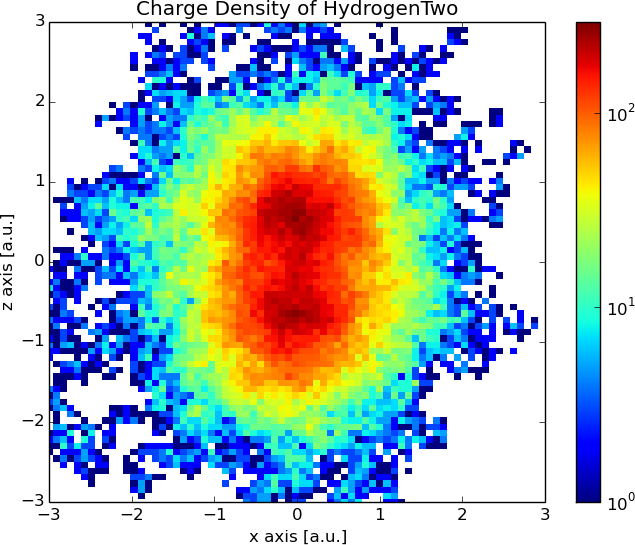
\includegraphics[width=0.45\linewidth]{../figures/used/OneBodyDensityHydrogenTwo}
			\protect\caption{Fill in $10^6$ cycles on both}
			\label{fig:chargeDensityHydrogenTwo}
		\end{figure}

	\subsubsection{Beryllium Molecule}
		\textbf{To be written tomorrow}
		\begin{figure}
			\centering 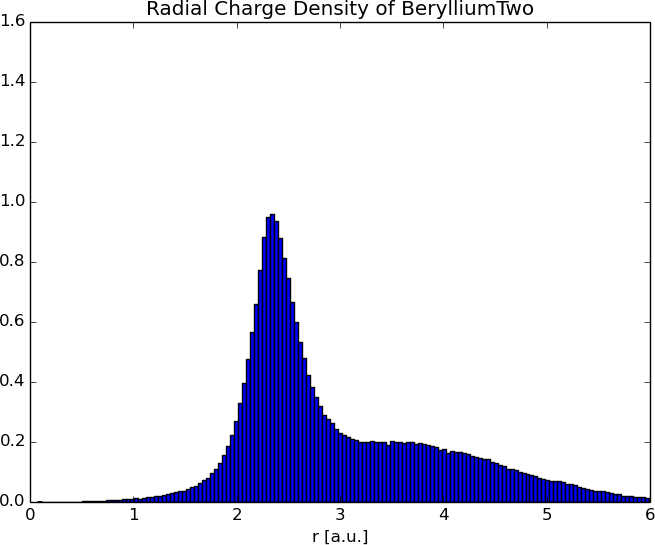
\includegraphics[width=0.45\linewidth]{../figures/used/ChargeDensityBerylliumTwo}
			\centering 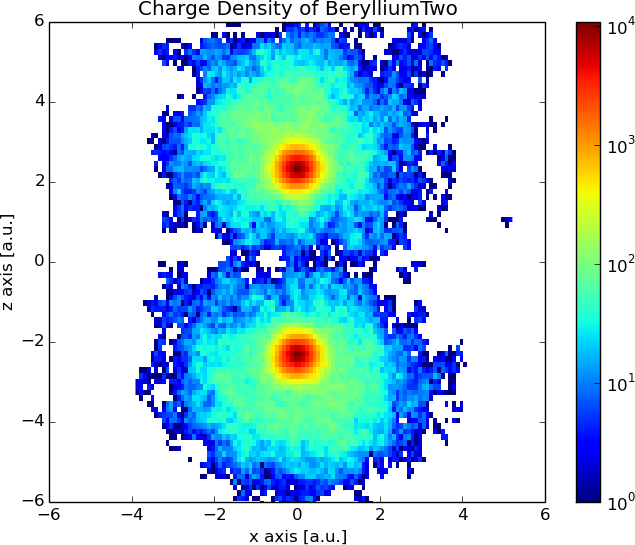
\includegraphics[width=0.45\linewidth]{../figures/used/OneBodyDensityBerylliumTwo}
			\protect\caption{Fill in  $10^6$ cycles on both  }
			\label{fig:chargeDensityBerylliumTwo}
		\end{figure}
